\documentclass{homework}
\usepackage{amsmath, amssymb}
\usepackage{enumitem}
\usepackage{float}
\usepackage{macros-common}
\usepackage{homework-lst}
\usepackage{hyperref}
\usepackage[top=1.5in,bottom=1.5in,left=1.4in,right=1.4in]{geometry}

\tcbset{listing only,colframe=bgcolor,
    colback=bgcolor,
    left=4pt,right=4pt,top=-2pt,bottom=-2pt,
    grow to left by=50pt,
    grow to right by=15pt,
    enlarge top by=10pt,
    enlarge bottom by=10pt,
    breakable}

\ExplSyntaxOn
\cfoot { \textcolor { homework_misccolor } { \hspace*{.8in}\sffamily \small \thepage } }
\ExplSyntaxOff
\title{Term Project\\[7pt] Implementation Report}
\subject{CS580 Computer Graphics}
\studentid{20170058}
\name{Keonwoo Kim}
\date{\today}

\begin{document}
\maketitle


\tableofcontents


\begin{figure}[H]
    \centering
    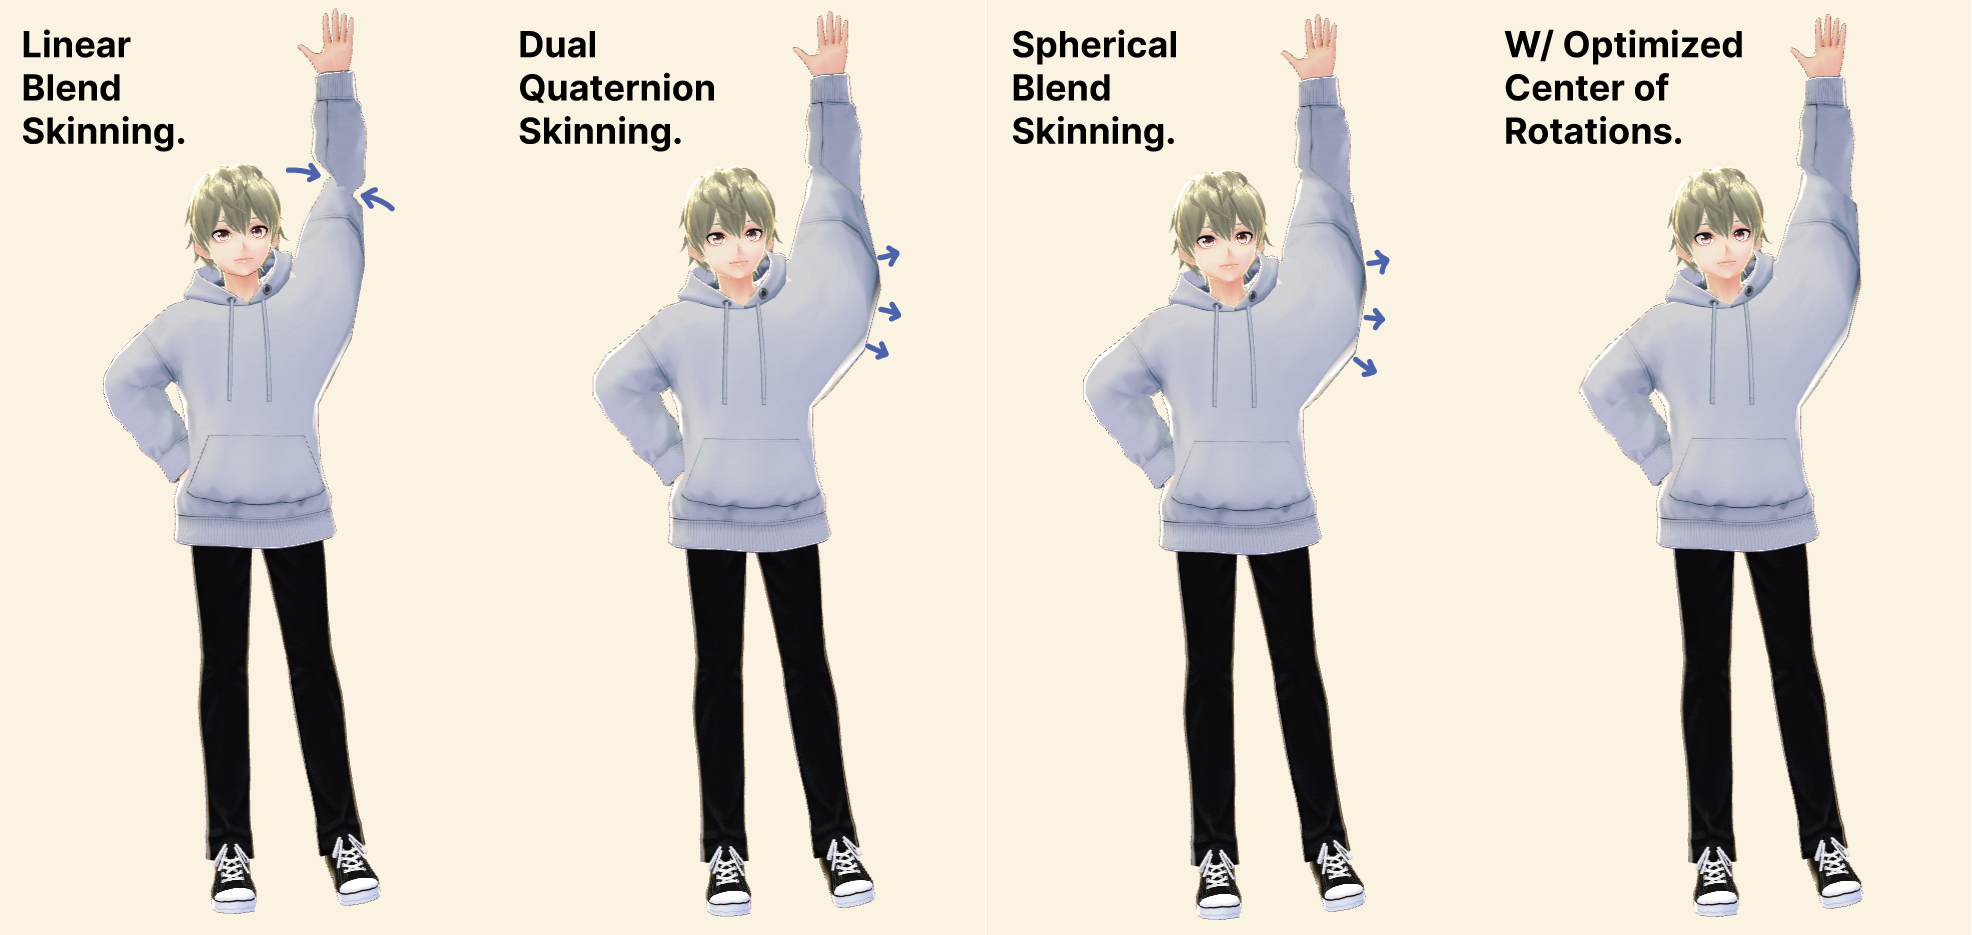
\includegraphics[width=\textwidth]{images/compare-skinning-methods.png}
    \caption{The comparison of skinning methods.}
\end{figure}

\setcounter{section}{-1}

\section{Introduction}
The project demonstrates various real-time skinning algorithms: linear blend skinning (LBS), dual quaternion skinning (DQS, or DLB) \cite{Kavan2008}, spherical blend skinning (SBS) \cite{Kavan2005}, and a variant of spherical blend skinning with optimized center of rotations (CoR) \cite{Le2016}.

The frontend web app is written mainly in vanilla \href{https://www.typescriptlang.org/}{TypeScript} and bundled by \href{https://webpack.js.org/}{webpack}. The backend server app is written in TypeScript using \href{https://www.fastify.io/}{\textit{fastify}}.

\section{Project Structure}
\subsection{Frontend}
The abstract class for an app is in \lst{src/App/Types}, and it is almost the same with one of \lst[js]{cs580} module. This app is created by the Redux reducer (\lst{src/Store/Reducer/App}) when the app state is changed from \lst{NONE} to \lst{MAIN} (\lst{src/index:6}.) Backend server status is managed by the reducer (\lst{src/Store/Reducer/Server}.)

The shaders used to skin vertices are defined in \lst{src/Shader/*}. \lst{substi} \lst{tuteShader} replaces \lst{#include<...>} directives by corresponding shader chunks until there are no replacements anymore. Common shader chunks are located in \lst{src/Shader/Chunk}, and other shader-specific chunks are in \lst{src/Shader/*/Chunk}.

\lst{wasm-blend} contains WebAssembly files providing SBS centers of rotation data, while it is not used in the project because it seems there are no advantage in performance over copying data from JS side to WASM side.

Static files including the model files are in \lst{dist/static} directory.

\subsection{Backend}
The backend project is in \lst{cor} directory. The default port number for the backend is \lst{9001}. The routes defined on the server (\lst{cor/src/server.ts}) are as follows:
\begin{itemize}
    \item [] \lst{GET /}: To check server availability.
    \item [] \lst{static /cache/* -> /*}: To serve cached optimized center of rotations binary data used by CoR.
    \item [] \lst{POST /}: To receive requests to generate CoR binary data.
    \item [] \lst{GET /:modelName}: To check if CoR data are generated completely for a model \lst{modelName}.
\end{itemize}

Workers that actually generate CoR data are in \lst{cor/src/worker.ts}.

\section{Load Models}
The format of the default model I used in this project is \href{https://vrm.dev/}{VRM}. VRM is based on glTF 2.0 and is specialized to represent humanoid models. To load VRM models into Three.js project using \href{https://github.com/pixiv/three-vrm}{three-vrm}, we need to load them as glTFs using GLTFLoader \lst{three/examples/jsm/loaders/GLTFLoader} and parse as VRMs using \lst{await VRM.from()}. To reduce time to traverse \lst{SkinnedMesh}es and \lst{ShaderMaterial}s in the model, they are stored in \lst{MainApp.vrms}. Finally, it tries to fetch optimized CoR data by long polling (\lst{MainApp.checkOptimizedCoRLongPolling()}.) When the data fetches are completed, CoR button on the side panel gets enabled.

\section{Linear Blend Skinning}
The default vertex shader for a VRM model is defined in \href{https://github.com/pixiv/three-vrm/blob/dev/packages/three-vrm/src/material/shaders/mtoon.vert}{three-vrm}, and it uses linear blend skinning (\lst{#include <skinning_vertex>}.) I mention here clearly that I did nothing to implement linear blend skinning, and \href{https://github.com/mrdoob/three.js/blob/dev/src/renderers/shaders/ShaderChunk/skinning_vertex.glsl.js}{the default shader} implements the linear blend skinning.

\begin{tcblisting}{listing options={language=glsl}}
// skinning_vertex.glsl
	vec4 skinVertex = bindMatrix * vec4( transformed, 1.0 );
	vec4 skinned = vec4( 0.0 );
	skinned += boneMatX * skinVertex * skinWeight.x;
	skinned += boneMatY * skinVertex * skinWeight.y;
	skinned += boneMatZ * skinVertex * skinWeight.z;
	skinned += boneMatW * skinVertex * skinWeight.w;
	transformed = ( bindMatrixInverse * skinned ).xyz;
\end{tcblisting}

\section{Helper Shader Chunks}
\subsection{Quaternions}

A quaternion is represented by a \lst[glsl]{vec4}. \lst{quatToMat3/4} converts a quaternion into a rotational matrix.

\begin{tcblisting}{listing options={language=glsl}}
// src/Shader/Chunk/quaternion.chunk.vert
mat3 quatToMat3( vec4 q ) {
  return mat3(
    // column 0
    1.0 - 2.0 * (q.y * q.y + q.z * q.z), 2.0 * (q.x * q.y + q.w * q.z),
    2.0 * (q.x * q.z - q.w * q.y),
    // column 1
    2.0 * (q.x * q.y - q.w * q.z),       1.0 - 2.0 * (q.x * q.x + q.z * q.z),
    2.0 * (q.y * q.z + q.w * q.x),
    // column 2
    2.0 * (q.x * q.z + q.w * q.y),       2.0 * (q.y * q.z - q.w * q.x),
    1.0 - 2.0 * (q.x * q.x + q.y * q.y)
  );
}
\end{tcblisting}

\lst{getQLERP} interpolates 4 quaternions w.r.t. the given weights. Here \lst{quatAntipodality} adjusts antipodality of quaternions, where $\mathbf q$ and $-\mathbf q$ represent the same 3D rotation while the interpolation results differ.

\begin{tcblisting}{listing options={language=glsl}}
// src/Shader/Chunk/quaternion.chunk.vert
float quatAntipodality( vec4 q1, vec4 q2 ) {
  return dot( q1, q2 ) < 0.0 ? -1.0 : 1.0||;
}

vec4 getQLERP(
  vec4 weights, vec4 quatX, vec4 quatY, vec4 quatZ, vec4 quatW
) {
  vec4 linearBlending = weights.x * quatX
      + weights.y * quatY * quatAntipodality( quatX, quatY )
      + weights.z * quatZ * quatAntipodality( quatX, quatZ )
      + weights.w * quatW * quatAntipodality( quatX, quatW );
  return linearBlending / length( linearBlending );
}
\end{tcblisting}

\subsection{Dual Quaternions}
A dual quaternion is represented by \lst{struct DualQuat} containing two quaternions \lst{rot} and \lst{transl}. \lst{getDLBMat4} blends 4 dual quaternions into one and converts it into a \lst[glsl]{mat4}. The algorithm is described in \cite[Algorithm 1]{Kavan2008}.

\begin{tcblisting}{listing options={language=glsl}}
// src/Shader/Chunk/dual_quaternion.chunk.vert
mat4 getDLBMat4(vec4 weights, DualQuat dqX, DualQuat dqY, DualQuat dqZ, DualQuat dqW) {
  // |\color{commentcolor}$\hat {\mathbf b}$| in the paper
  DualQuat linearBlending;
  linearBlending.rot = /* omitted */;
  linearBlending.transl = /* omitted */;

  float linearBlendingNorm = length( linearBlending.rot );
  vec4 r = linearBlending.rot / linearBlendingNorm; // |\color{commentcolor}$\mathbf c_0$| in the paper
  vec4 e = linearBlending.transl / linearBlendingNorm; // |\color{commentcolor}$\mathbf c_\varepsilon$| in the paper
  return mat4( /* omitted */ );
}
\end{tcblisting}


\section{Dual Quaternion Skinning}
With \lst{getDLBMat4} above, dual quaternion skinning is done very easily. First, bone matrices in dual quaternion form is given as uniform variables, packed in a \lst[js]{THREE.DataTexture}. The algorithm for \lst{DualQuaternion.fromMat4} is described in \cite[Equation (25)]{Kavan2008}.

\begin{tcblisting}{listing options={language=js}}
// src/App/Main
switch (this.skinningType) {
case SkinningType.DUAL_QUATERNION: {
  const dualQuatBoneArray = _.range(mesh.skeleton.bones.length)
    .map((i) => DualQuaternion.fromMat4(
                  new THREE.Matrix4()
                    .fromArray(mesh.skeleton.boneMatrices, 16 * i)
                    .premultiply(mesh.bindMatrix)
                    .multiply(mesh.bindMatrixInverse)))
    .map((dq) => dq.toArray()).flat();

  const dataTexture = material.uniforms.dualQuatBoneTexture?.value
    as THREE.DataTexture;
  dataTexture.image.data.se||t(dualQuatBoneArray);
  dataTexture.needsUpdate = true;
  break;
}
\end{tcblisting}

\begin{tcblisting}{listing options={language=glsl}}
// src/Shader/DualQuaternion/Chunk/dual_quaternion_skinnormal.chunk.vert
mat4 skinMatrix = getDLBMat4( skinWeight, boneDqX, boneDqY, boneDqZ, boneDqW );
objectNormal = vec4( skinMatrix * vec4( objectNormal, 0.0 ) ).xyz;
#ifdef USE_TANGENT
  objectTangent = vec4( skinMatrix * vec4( objectTangent, 0.0 ) ).xyz;
#endif |\ |
// src/Shader/DualQuaternion/Chunk/dual_quaternion_skinning.chunk.vert
transformed = ( skinMatrix * vec4( transformed, 1.0 ) ).xyz;
\end{tcblisting}

\allowdisplaybreaks
\section{Spherical Blend Skinning}
To implement spherical blend skinning, one needs to solve the following least squares problem for each vertex $\mathbf v$:
\begin{align*}
    \text{minimize} &\sum_{\substack{i < j \\w_\mathbf v^{(i)} \ne 0 \ne w_\mathbf v^{(j)} }} \left\| (M^{(i)} - M^{(j)})\binom{\mathbf r_\mathbf v}{1}\bigg|_{xyz} \right\|^2 =\sum_{\substack{i < j \\w_\mathbf v^{(i)} \ne 0 \ne w_\mathbf v^{(j)} }} \| (R^{(i)} - R^{(j)})\mathbf r_\mathbf v - (\mathbf t^{(j)} - \mathbf t^{(i)}) \|^2 
 \\&= \left\| \underbrace{\begin{bmatrix}\vdots \\R^{(i)} - R^{(j)} \\ \vdots\end{bmatrix}_{3\binom n 2\times 3}}_{\texttt{svdCoeff}^\dagger} \mathbf r_{\mathbf v} - \underbrace{\begin{bmatrix}\vdots \\\mathbf t^{(j)} - \mathbf t^{(i)} \\ \vdots\end{bmatrix}_{3\binom n 2\times 1} }_{\texttt{svdConst}^\dagger}\right\|^2
\end{align*}
where $M^{(i)} = \begin{bmatrix}R^{(i)} & \mathbf t^{(i)}\\ \mathbf 0&1\end{bmatrix}$ is the (complete) bone matrix (after premultiplying the bind matrix and postmultiplying the inverse of it) the $i$-th bone, $w_{\mathbf v}^{(i)}$ is the skin weight of $\mathbf v$ to the $i$-th bone, and $n$ is the number of bones to which $\mathbf v$ is bound with nonzero skin weight.

The computation is done at each frame using SVD ($^\dagger$ Refer to \lst{src/App/Main:L349-475}). To reduce the number of computation, the result $\mathbf r_\mathbf v$, which depends on the set of bone indices $i$ where $w_\mathbf v^{(i)}$ is nonzero, is cached into \lst{centerOfRotationTable}, and used for other vertices. Finally, they are wrapped into an attibute and passed to the vertex shader. Then the final transform $\mathbf v \mapsto Q(\mathbf v - \mathbf r_\mathbf v) + \sum w_\mathbf v^{(i)}M^{(i)}\mathbf r_\mathbf v$ is constructed where $Q$ is the QLERPed rotational matrix of $R^{(i)}$'s. Note for \lst[glsl]{vec3}s the transform becomes $\mathbf n \mapsto Q\mathbf n$.

Besides the center of rotation attribute, (the rotational parts of) bone matrices in quaternion form are also given as a uniform variable, packed in a \lst[js]{THREE.DataTexture} (\lst{src/App/Main:L324-345}).

\begin{tcblisting}{listing options={language=glsl}}
// src/Shader/SphericalBlendSkinning/Chunk/spherical_blend_skinnormal.chunk.vert
vec4 qlerped = getQLERP( skinWeight, boneQuatX, boneQuatY, boneQuatZ, boneQuatW );
mat3 skinMatrix3 = quatToMat3( qlerped );
objectNormal = skinMatrix3 * objectNormal;
#ifdef USE_TANGENT
  objectTangent = skinMatrix3 * objectTangent;
#endif |\ |

// src/Shader/SphericalBlendSkinning/Chunk/spherical_blend_skinning.chunk.vert
vec3 transl = vec3( 0.0 );
transl += vec3( boneMatX * vec4( centerOfRotation, 1.0 ) ) * skinWeight.x;
transl += vec3( boneMatY * vec4( centerOfRotation, 1.0 ) ) * skinWeight.y;
transl += vec3( boneMatZ * vec4( centerOfRotation, 1.0 ) ) * skinWeight.z;
transl += vec3( boneMatW * vec4( centerOfRotation, 1.0 ) ) * skinWeight.w;

transformed = skinMatrix3 * ( transformed - centerOfRotation ) + transl;
\end{tcblisting}

\section{With Optimized Center of Rotations}
The shader code is the same with SBS. The only difference is the content of the attribute \lst{centerOfRotation}. It is first stored in \lst{MainApp.optimizedCoRBuffers} as \lst{Float32Array}s after fetching from the server, and passed into the shader if the skinning type is CoR. The advantage of this method is that there is no need to alter the vertex attribute at every render, since the center of rotations do not depend on bone matrices, but only on vertices (on rest pose), triangles, and skin weights, which are not changed over time. So, the attribute is set when the skinning type is changed (\lst{src/App/Main:L273-278}).

The paper \cite{Le2016} introduces methods to optimize the baking time, however I did not implement those as it does not take that much time to execute. (To reproduce, click generate optimized CoR data button. Caution: the computer may become super laggy.) The code for generating optimized center of rotations is very straightforward to \cite[Equation (4)]{Le2016}. See \lst{cor/src/worker.ts}.

\begin{tcblisting}{listing options={language=js}}
// cor/src/worker.ts
const approxOptimalCoRArray = _.range(vertices.length / 3)
  .map((vertexIndex) => {
    const wi = skinWeights[vertexIndex];
    const numerator = [0, 0, 0];
    let denominator = 0;

    _.chunk(triangleIndices, 3).forEach(([ia, ib, ic]) => {
      const va = getVertex(ia);
      const vb = getVertex(ib);
      const vc = getVertex(ic);
      const wa = skinWeights[ia];
      const wb = skinWeights[ib];
      const wc = skinWeights[ic];
      const wav = averageSkinWeight(wa, wb, wc);
      const vav = averageVertex(va, vb, vc);

      const area = getTriangleArea(va, vb, vc);
      const coeff = similarity(wi, wav) * area;
      numerator[0] += coeff * vav[0];
      numerator[1] += coeff * vav[1];
      numerator[2] += coeff * vav[2];
      denominator += coeff;
    });

    if (denominator === 0) {
      return [0, 0, 0] as Vertex;
    }

    return numerator.map((x) => x / denominator) as Vertex;
  })
  .flat();
\end{tcblisting}


\section{Discussion}
\subsection{Performances}
LBS and DQS both showed good performances without any lag on a consumer computer. CoR had a subtle delay probably because of passing large attributes, but it seems okay in general. However, SBS had a severe performance issue. It gets worse as it tries to do singular value decomposition in the browser at real-time, which is slower than native environments.

\subsection{Artifacts}

\begin{figure}[H]
    \centering
    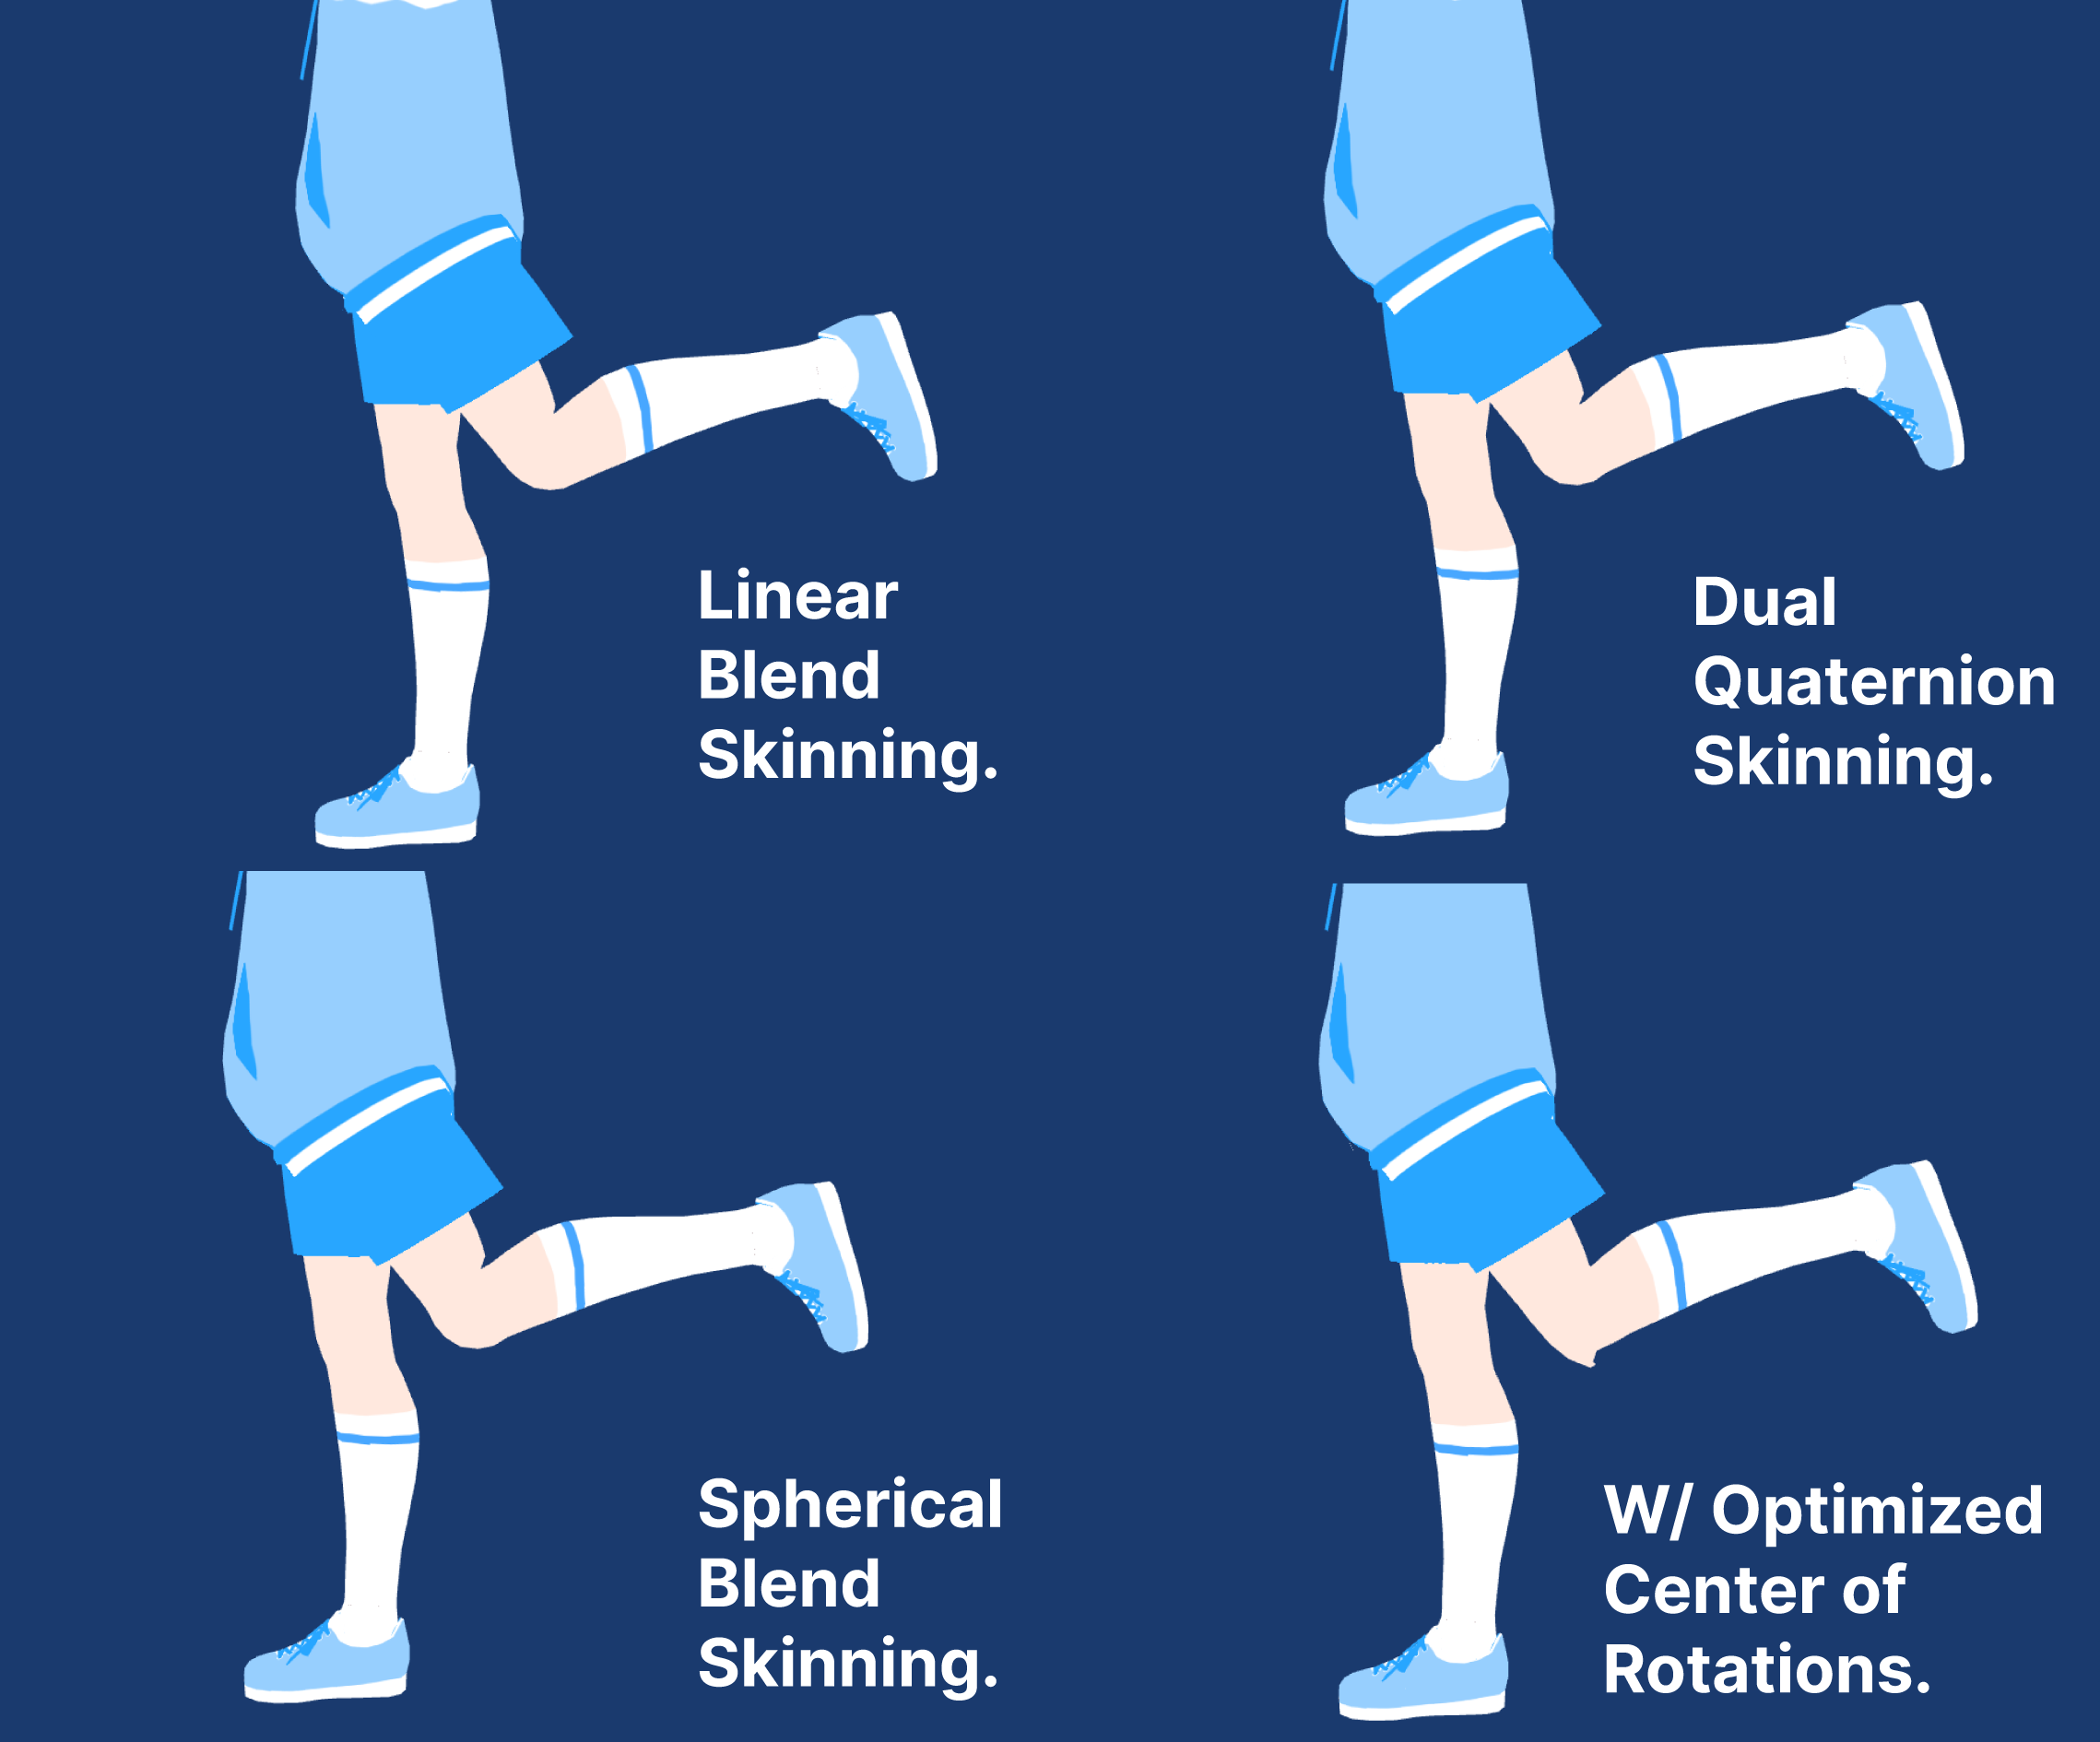
\includegraphics[width=0.7\textwidth]{images/artifact2.png}
    \caption{DQS and SBS have a crease and joint bulging effect, and CoR shows a discontinuous knee mesh.}
\end{figure}

Figures 1 and 2 show some artifacts of each method. First, the candy wrapper artifact is shown in LBS, when an arm is twisted (rotated about the arm direction.) And nonlinear methods, especially DQS ans SBS, show bulging artifacts. Moreover, as indicated in \cite[Figure 4]{Le2016}, with DQS or SBS, the knee part is bulged while there is a crease near the back of the knee which is clearer than LBS. However, a discontinuity is found with CoR, which is because the leg does not consist of a single mesh in my opinion. Since the optimized center of rotations is obtained for each mesh, regardless of neighbor meshes.

\subsection{Unintended Bugs}
\begin{figure}[H]
    \centering
    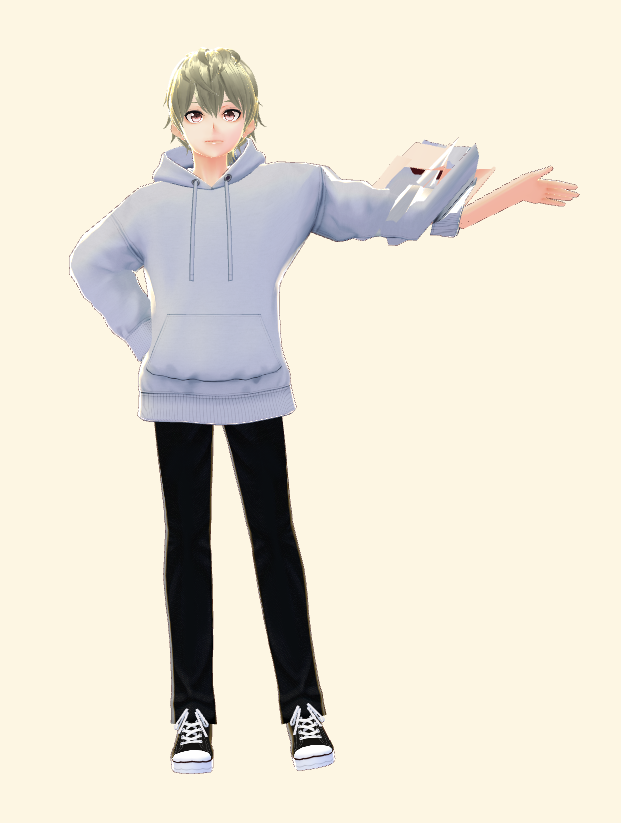
\includegraphics[width=0.4\textwidth]{images/artifact1.png}
    \caption{An unintended bug producing weird results.}
\end{figure}
When running SBS and CoR at a high animation speed, the results seem very strange. And these artifacts disappear when one `pauses' the animation by pressing Pause button. With some analyses, I think it is because the meshes and materials are separated and the app traverses the object sequentially. Especially, when each render step contains heavy operations such as large data copy or singular value decomposition, sequential update of attributes affect the actual results. It is probably the reason why the result is normal when the animation is paused by `Pause' button (which internally keeps to render) but not when the execution is paused using browser debugger.






\bibliographystyle{alpha}
\bibliography{assignment-term-report}
\end{document}